\documentclass[a4paper, 12pt]{report}

%%%%%%%%%%%%
% Packages %
%%%%%%%%%%%%

\usepackage[english]{babel}
\usepackage{packages/sleek}
\usepackage{packages/sleek-title}
\usepackage{packages/sleek-theorems}
\usepackage{packages/sleek-listings}
\usepackage{tikz}
\usetikzlibrary{decorations.pathmorphing}

%%%%%%%%%%%%%%
% Title-page %
%%%%%%%%%%%%%%

\title{Vibration Engineering Notes}
\subtitle{Textbook: Engineering Vibration, 4th Edition, Daniel J. Inman}
\author{\textit{Author}\\Philip \textsc{Ligthart}}
\date{\today}

%%%%%%%%%%
% Macros %
%%%%%%%%%%

\def\tbs{\textbackslash}

%%%%%%%%%%%%
% Document %
%%%%%%%%%%%%

\begin{document}
    \maketitle
    \romantableofcontents

    \chapter{Chapter 1 - Introduction to vibration and free response}

      \begin{fmd-definition}{Degree of freedom}
        The degree of freedom of a system is the minimum number of displacement coordinates needed to represent the position of the systems mass at any instant of time.
      \end{fmd-definition}

      \begin{fmd-definition}{Free response}
        Free response refers to analysing the vibration of a system resulting from a non-zero inital displacement and/or velocity of the system with no external force or moment applied.
      \end{fmd-definition}
  
      \section{The spring-mass model}
        The fundamental kinematic quantities used to describe the motion of a particle are displacement, velocity, and acceleration vectors.

        \begin{fmd-definition}{Kinematic}
          Kinematic quantities are those that describe the motion of a particle without regard to the forces that cause the motion.
        \end{fmd-definition}
        
        \begin{figure}
          \centering
          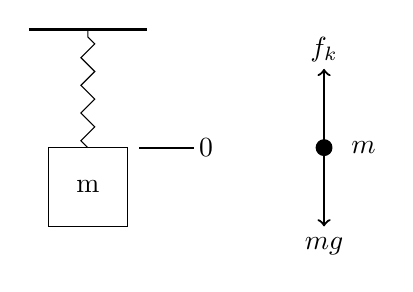
\begin{tikzpicture}
            % single DOF mass-spring system
            \draw[thick] (-0.25,2.5) -- (1.25,2.5);
            \draw (0,0) rectangle (1,1);
            \node at (0.5,0.5) {m};
            \draw[decorate,decoration=zigzag] (0.5,1) -- (0.5,2.5);
            \draw[thick] (1.15,1) -- (1.85,1);
            \node at (2,1) {0};
            % draw a point mass
            \draw[fill] (3.5,1) circle (0.1);
            \node at (4,1) {$m$};
            \draw[thick,->] (3.5,1) -- (3.5,2); % kx
            \node at (3.5,2.25) {$f_k$};
            \draw[thick,->] (3.5,1) -- (3.5,0); % mg
            \node at (3.5,-0.25) {$mg$};

          \end{tikzpicture}
          \caption{Single degree of freedom mass-spring system}\label{fig:single-dof-mass-spring}
        \end{figure}



\end{document}
